\chapter{Blur level set}
During the reconstruction of the surface all methods, in one form or another (depending on the level set computation approach), are using particle displacement information,. In the SPH based fluid simulation frameworks the displacement is usually irregular, thus small gaps can be formed. This gaps are threated as undesirable low frequency noise. The comparison of the surface reconstruction based on regular and irregular displacement of the particles is in the Figure \ref{fig:rec_vs_displacement}.
\begin{figure}[H]
	\begin{center}
		\begin{subfigure}[b]{0.6\textwidth}
			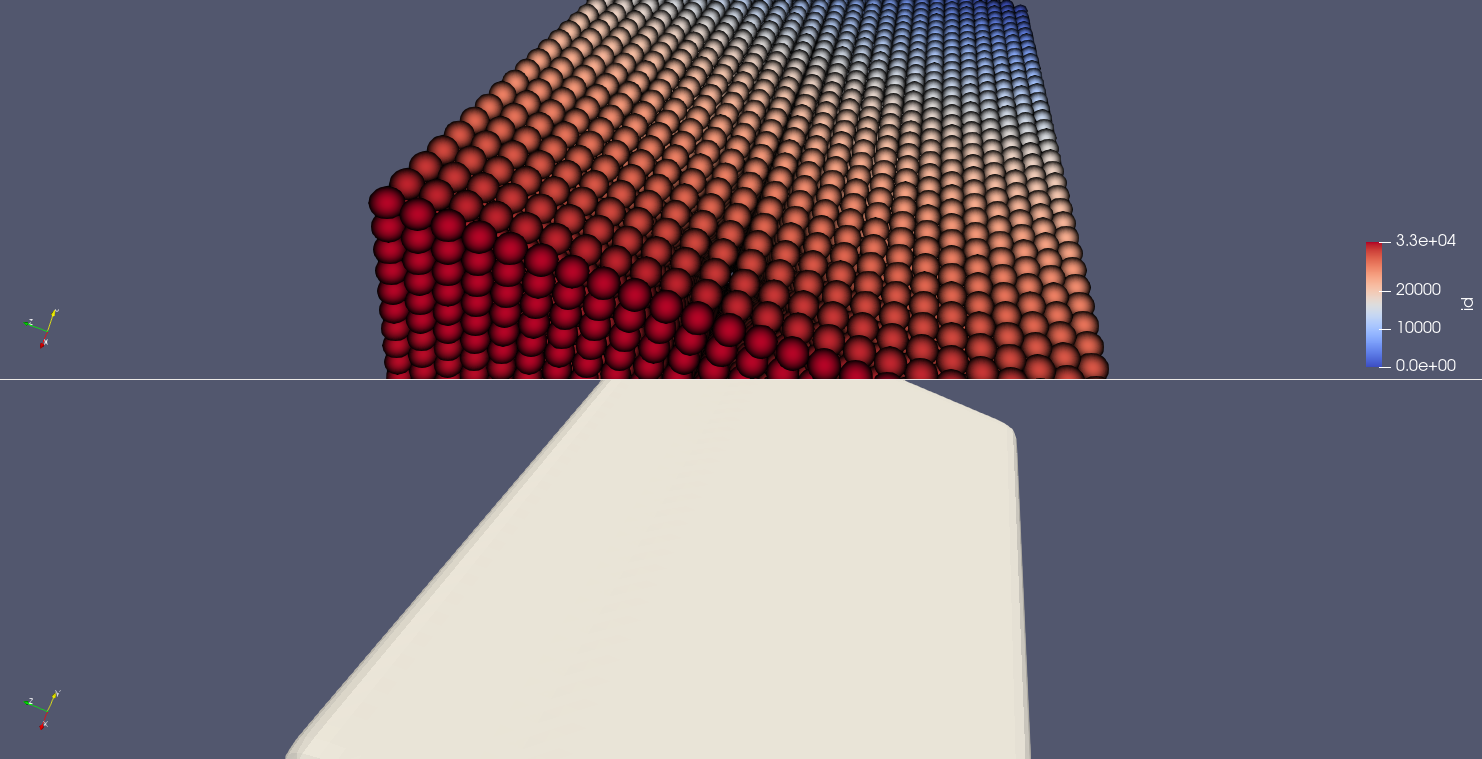
\includegraphics[width=\textwidth]{figures/FlatSurfaceWsParticleDisplacement.png}
			\caption{Regularly displaced particles}
		\end{subfigure}
		\begin{subfigure}[b]{0.6\textwidth}
			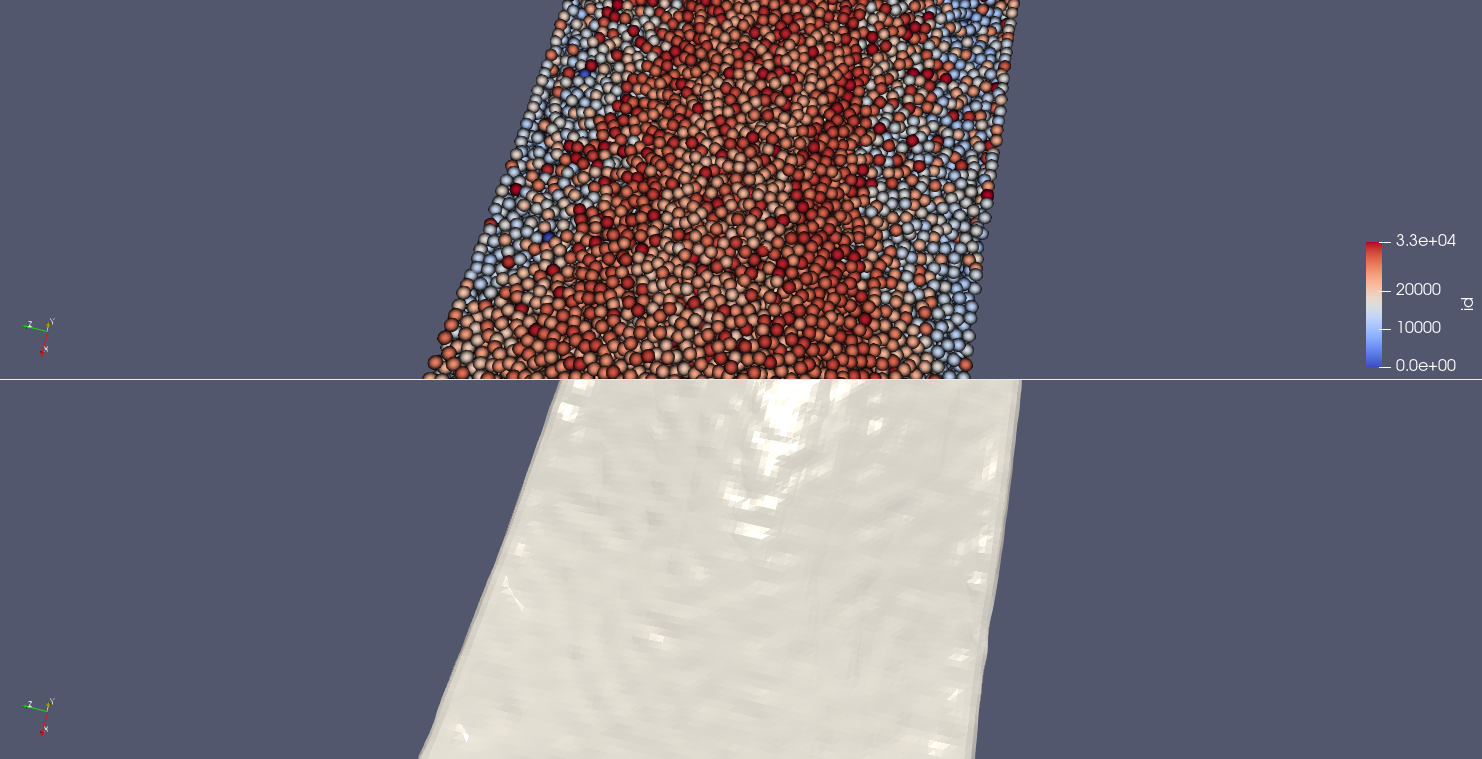
\includegraphics[width=\textwidth]{figures/NonFlatSurfaceWsParticleDisplacement.png}
			\caption{Irregularly displaced particles}
		\end{subfigure}
	\end{center}
	\caption{displacement of particles vs surface quality comparison}
	\label{fig:rec_vs_displacement}
\end{figure}
The main goal of this thesis is to develop a method, which will smooth out a high frequency bumps on flat surface areas, preserving the surface features. The first idea, that was applied to achieve this goal is simple blurring technique, which is extensively used in computer graphics, such as Gaussian Blur, Median blur, Bilateral blur or other image filtering techniques. In this chapter Blur-based method will be proposed to achieve the given goal. 
\section{Algorithm description}
Blur method was incorporated into the research framework according to the class hierarchy in Figure \ref{fig:class-diagam}. According to the class diagram the method inherits underlying base method (in our case its Dencity Based, Zhu and Bridson or Solenthaler metods), on top of which computed level set is blurred.  Algorithm \ref{alg:blur_alg} shows the pseudo-code fpr \emph{updateLevelSet()}.
\begin{algorithm}[H]
	\begin{algorithmic}
		\State $levelSet \gets  BaseClass::initialLevelSet$
		\For{$i \in [0, blurIterations]$}
			\State blurLevelSet(levelSet);
		\EndFor
	\end{algorithmic}
	\caption{$updateLevelSet()$ for level set blurring method}
	\label{alg:blur_alg}
\end{algorithm}
According to Algorithm \ref{alg:blur_alg} blurring of the level set could be performed arbitrary number of times. The influence of number of iterations will be explained in further section.

The \emph{blurLevelSet()} pesudo-code is explained in Algorythm \ref{alg:blur_level_set}
\begin{algorithm}[H]
	\begin{algorithmic}
		\ForAll{$vtx \in MC\_CellDomain$}
			\State $neighbors \gets getNeighbourVertices(vtx);$
			\State $blurredLevelSetValue \gets 0$
			\ForAll{$nbVtx \in neighbors$}
				\State $blurredLevelSetValue\gets blurredLevelSetValue + levelSet[neighborVertex]$
			\EndFor
			\State $blurredLevelSetValue\gets\dfrac{blurredLevelSetValue}{sizeof(neighbors)}$
			\State $sf\gets computeSmoothingFactor()$
			\State $blurredLevelSet[vtx]\gets levecSet[vtx] * (1 - sf) + sf * blurredLevelSetValue;$
		\EndFor
	\end{algorithmic}
	\caption{$updateLevelSet()$ for level set blurring method}
	\label{alg:blur_level_set}
\end{algorithm}
The final blurred level set value in Algorythm \ref{alg:blur_level_set} is a wighted sum between the computed blur level set value and initial level set value.
\subsection{Smoothing factor}
The smoothing factor is a value that determines how much new, blurred level set value will contain initial level set value (weighted sum of blurred level set value and initial level set value). As described in \ref{alg:blur_level_set} level set value is updated according to the Equation \ref{eq:level_set_value}.
\begin{equation}
newLS = oldLS \cdot (1 - sf) + blurLS \cdot sf \label{eq:level_set_value}
\end{equation}
In Equation \ref{eq:level_set_value} $sf$ is a smoothing factor or a weight. The smoothing factor itself is calculated according to equation \ref{eq:smooth_factor}.
\begin{equation}
	sf_{vtx} = -1 \cdot (1 - min(1, \dfrac{bsf \cdot fp_{vtx}}{maxFp})^2)^{10} + 1 \label{eq:smooth_factor}
\end{equation}
where:
\begin{conditions}
	vtx & vertex for which the smoothing factor is computed\\
	fp_{vtx} & number of neighbor fluid particles within support radius from vtx\\
	maxFp & maximum possible fluid particles that can be in the neighborhood of the vertex \\
	bsf & base support factor (use defined)
\end{conditions}
The smoothing factor formula was designed such that it should be maximal for vertices that contains full fluid particles set and minimum where number of fluid particles limits to zero. The motivation to apply such smoothing factor comes from the problem of the blurring algorythm. If we apply blur algorithm uniformly in to all MC vertex domain,  blur will smooth out the features in a thin areas and in the areas with small set of particles (droplets or splashes). Figure \ref{fig:smoothing_factor_influence} shows the problem off application of the blur algorithm w.o. application of smoothing factor.


\begin{figure}[H]
	\begin{center}
			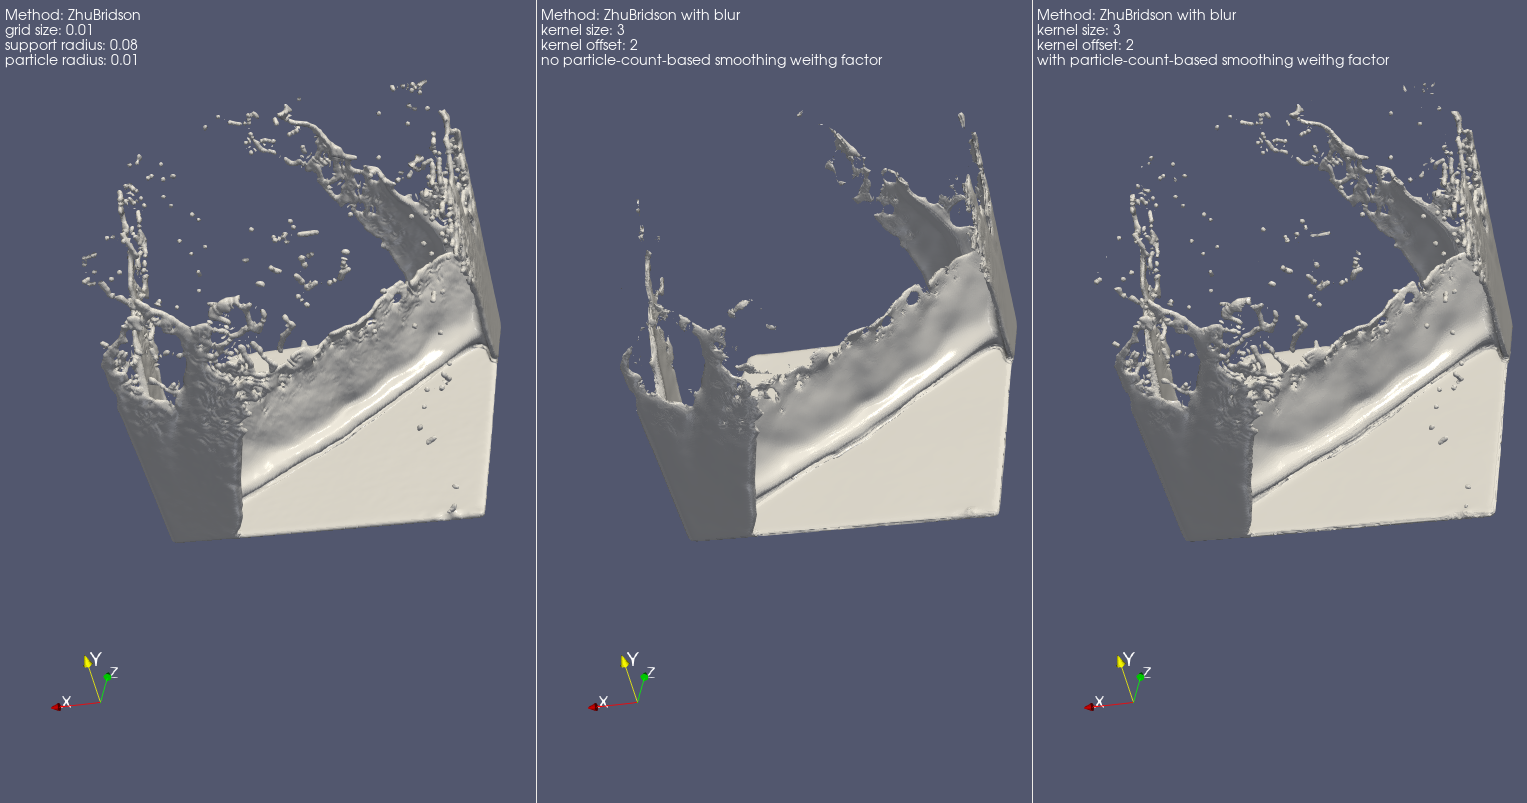
\includegraphics[width=\textwidth]{figures/View2.png}		
	\end{center}
	\caption{Leftmost is initial Zhu and Bridson reconstruction, middle - blur reconstruction w.o. smoothing factor application, rightmost - blur reconstruction with usage of smoothing factor}
	\label{fig:smoothing_factor_influence}
\end{figure}

The idea of blurring using smoothing factor is to blur level set as much as possible in the areas where surface of fluid is normal flat surface, and to apply less blur in areas, where set of MC cells lacks fluid particles. Suppose the general case in Figure \ref{fig:sf_example}. In the figure red and yellow grid vertices contains full and half set of particles respectively. Level set values of the grid points are supposed to be blurred as much as possible.
\begin{figure}[H]
	\begin{center}
		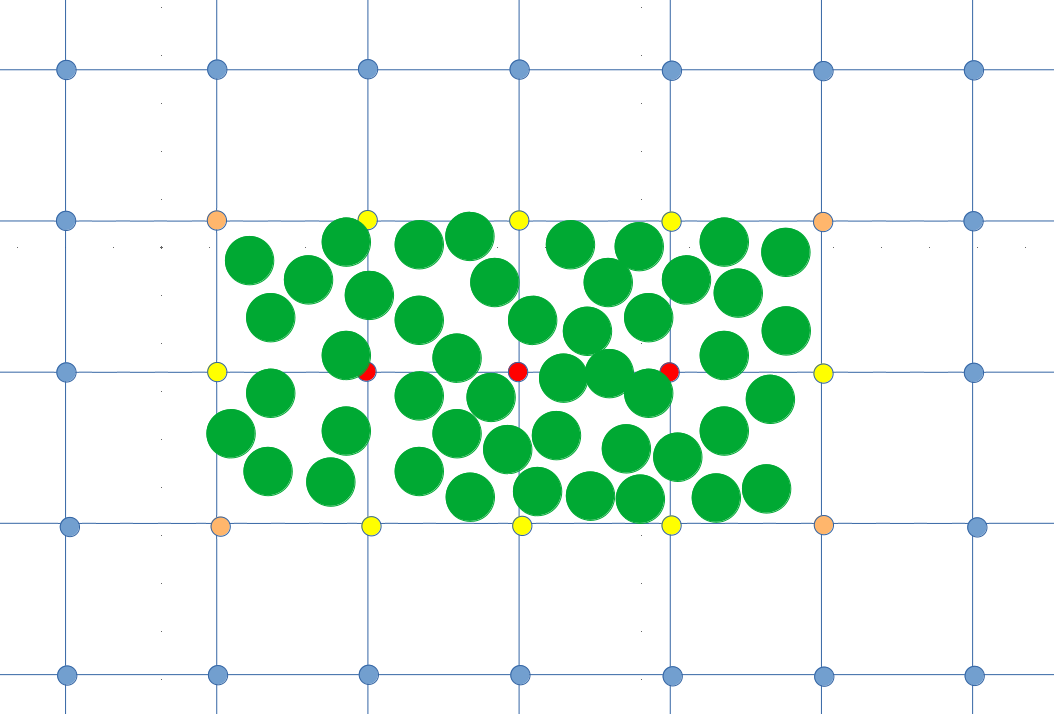
\includegraphics[width=0.5\textwidth]{figures/SmoothingFactorPictureExplenation.png}		
		\caption{Green circles are fluid particles, red - MC cells with full set of fluid particles in the neighborhood, yellow -  MC cells with half set of fluid particles in the neighborhood, orange - MC cells with quarter set of fluid particles in the neighborhood, blue - MC cells with no fluid particles in the neighborhood}
		\label{fig:sf_example}
	\end{center}
\end{figure}
Applying blur to the level set vertices that are inside the fluid (and all its neighbor cells are also inside the fluid) will not change the level set value too much as soon all vertices that has full set of fluid particles in the neighborhood will have similar level set values. 
For the MC vertices that are near the corners the 75\% of the neighbor vertices are outside the fluid, which will bias the vertex outside the fluid, thus the fluid will shrink. This is also relevant for the thin areas and splashes.\\
At the figure \ref{fig:blur_thin_area} the effect of applying blur in the thin area and in the corners can be observed. The flat surface is smoothed out, but at the same time surface at the thin and splash areas is degraded, some small features/droplets are lost
\begin{figure}[h]
	\begin{center}
		\begin{subfigure}[b]{\textwidth}
			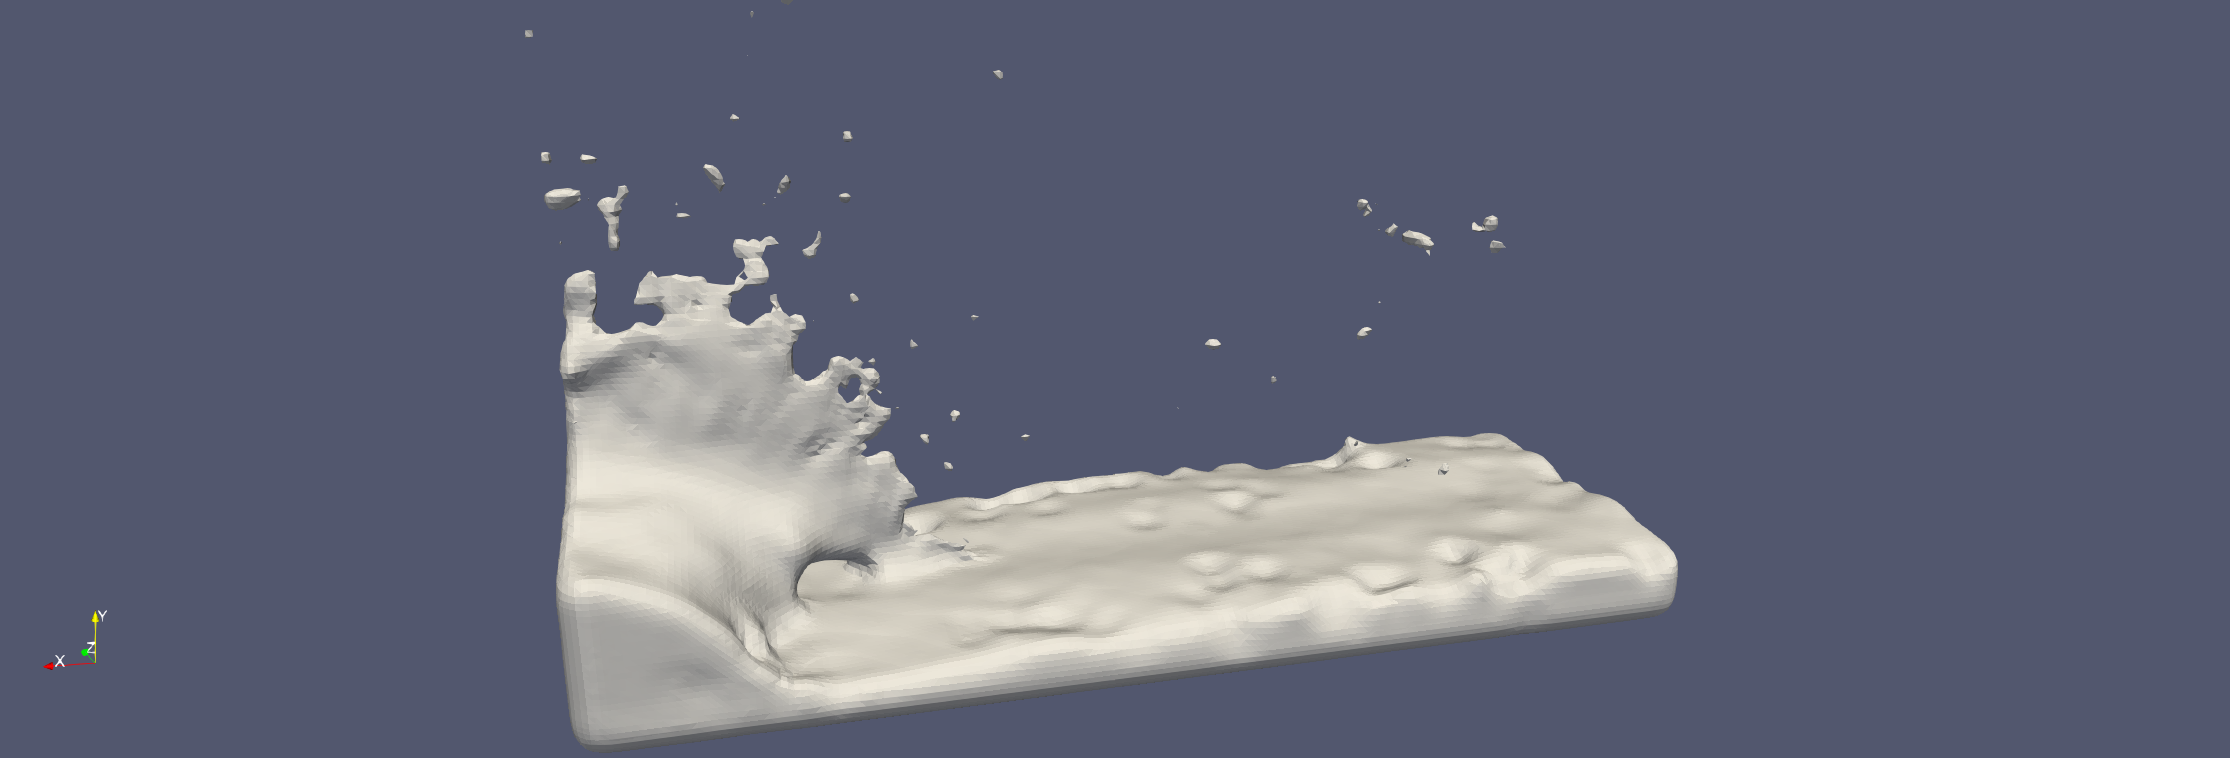
\includegraphics[width=\textwidth]{figures/DenvityBasedSplashArea.png}
			\caption{Density based surface reconstruction with blur (smoothing factor is not applied)}
		\end{subfigure}
		\begin{subfigure}[b]{\textwidth}
			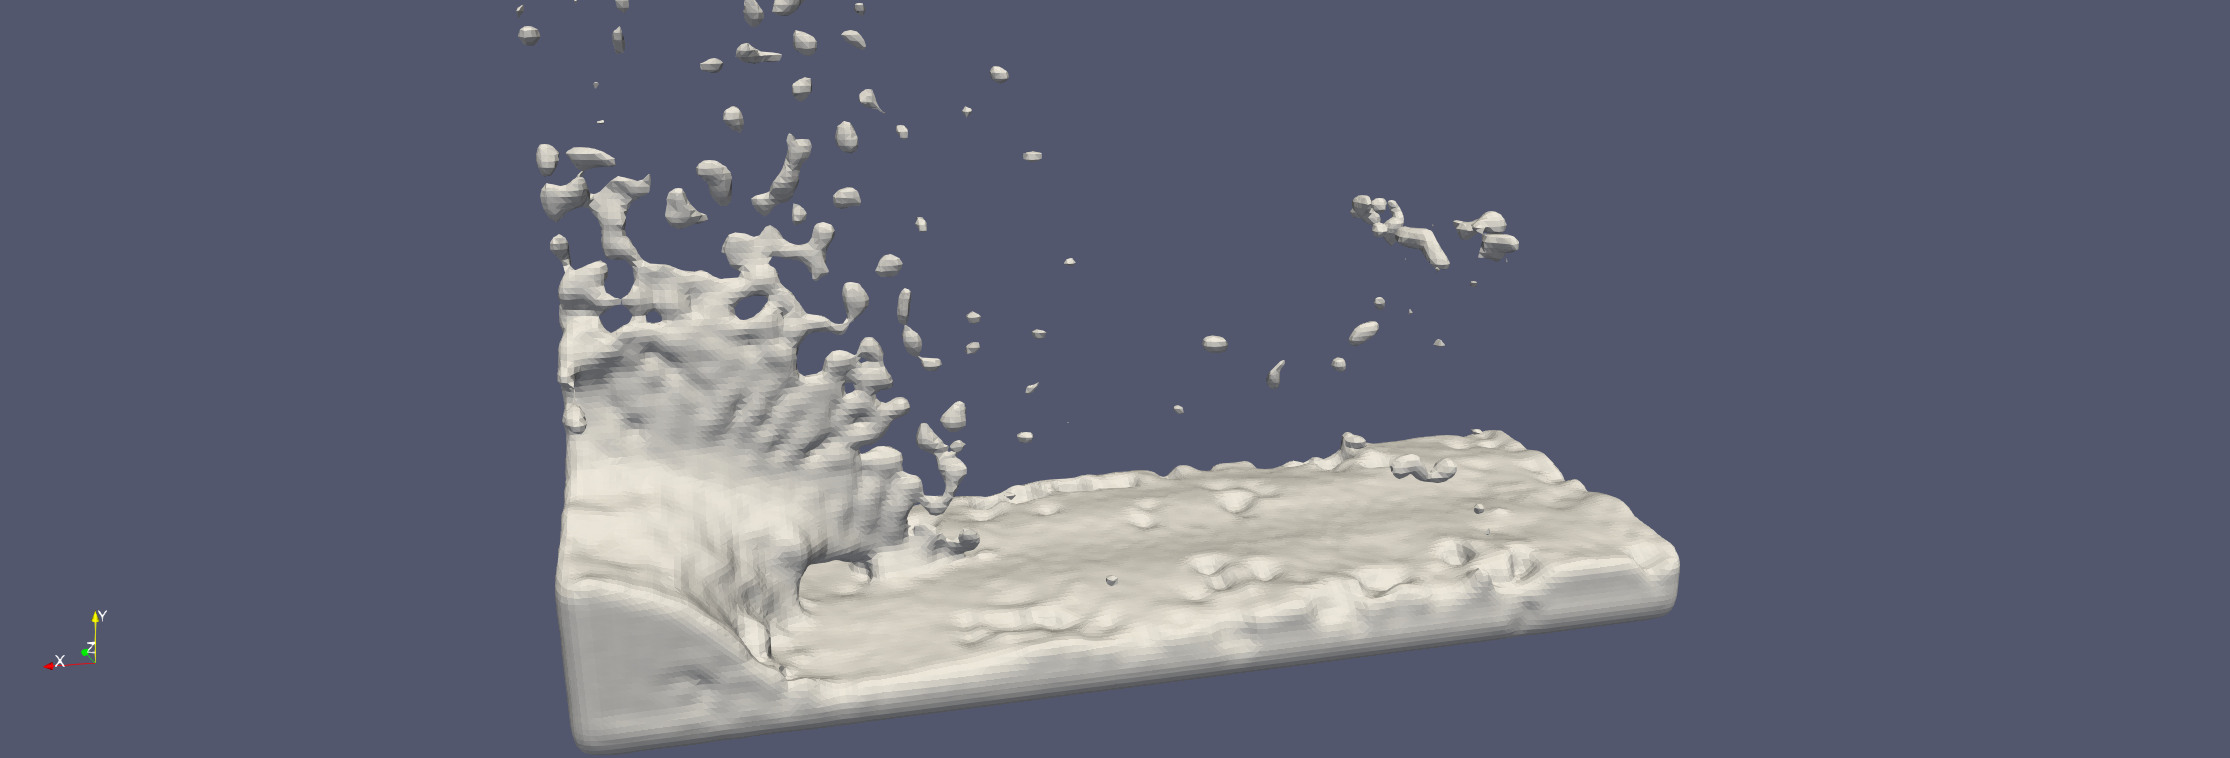
\includegraphics[width=\textwidth]{figures/DenvityBlurredSplashArea.png}
			\caption{Density based surface reconstruction}
		\end{subfigure}
	\end{center}
	\caption{Comparison of original reconstruction method and blurred reconstruction without application of smoothing factor}
	\label{fig:blur_thin_area}
\end{figure}
In contrast to this application of the smoothing factor smooths out the flat surface areas, but still preserves small feature areas (see Figure \ref{fig:blur_thin_area_with_sf}).
\begin{figure}[h]
	\begin{center}
		\begin{subfigure}[b]{\textwidth}
			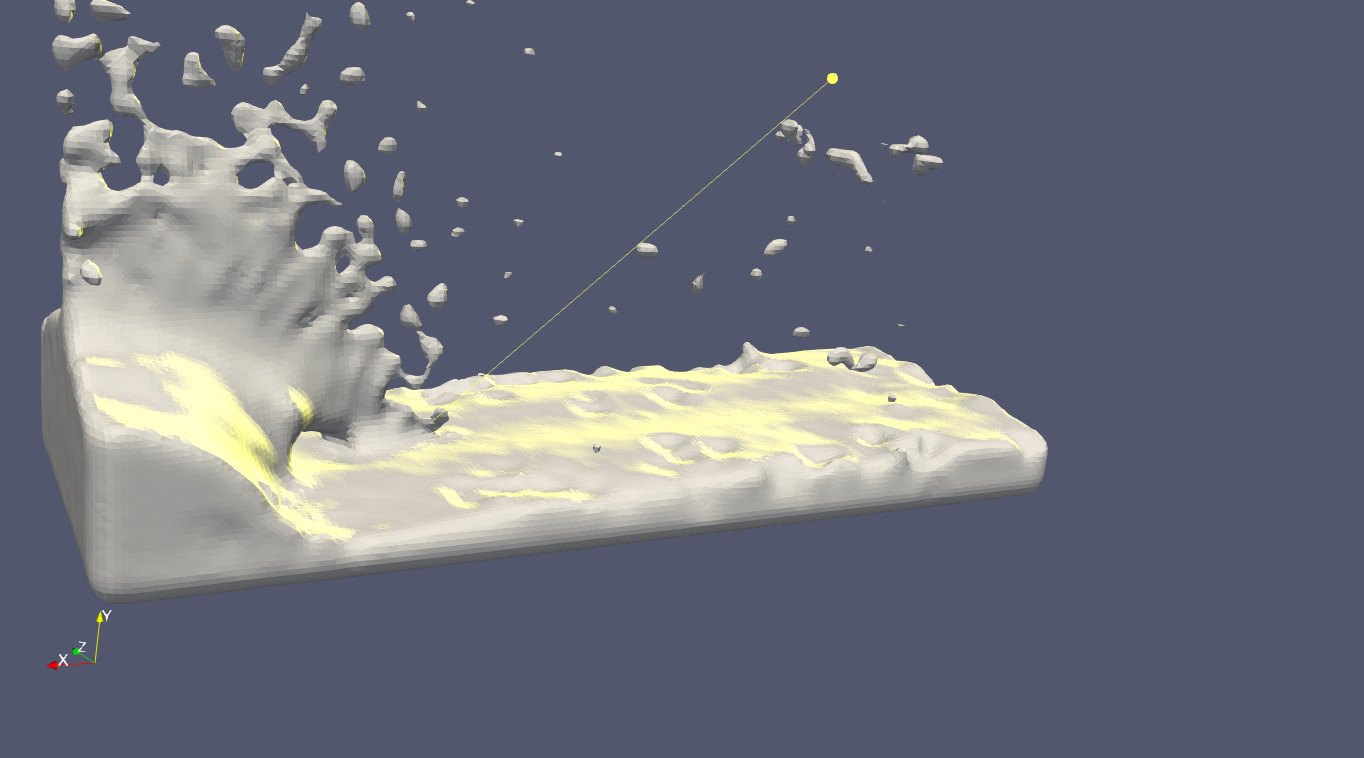
\includegraphics[width=\textwidth]{figures/DenvityBasedSplashArea2.png}
			\caption{Density based surface reconstruction with blur (smoothing factor is applied)}
		\end{subfigure}
		\begin{subfigure}[b]{\textwidth}
			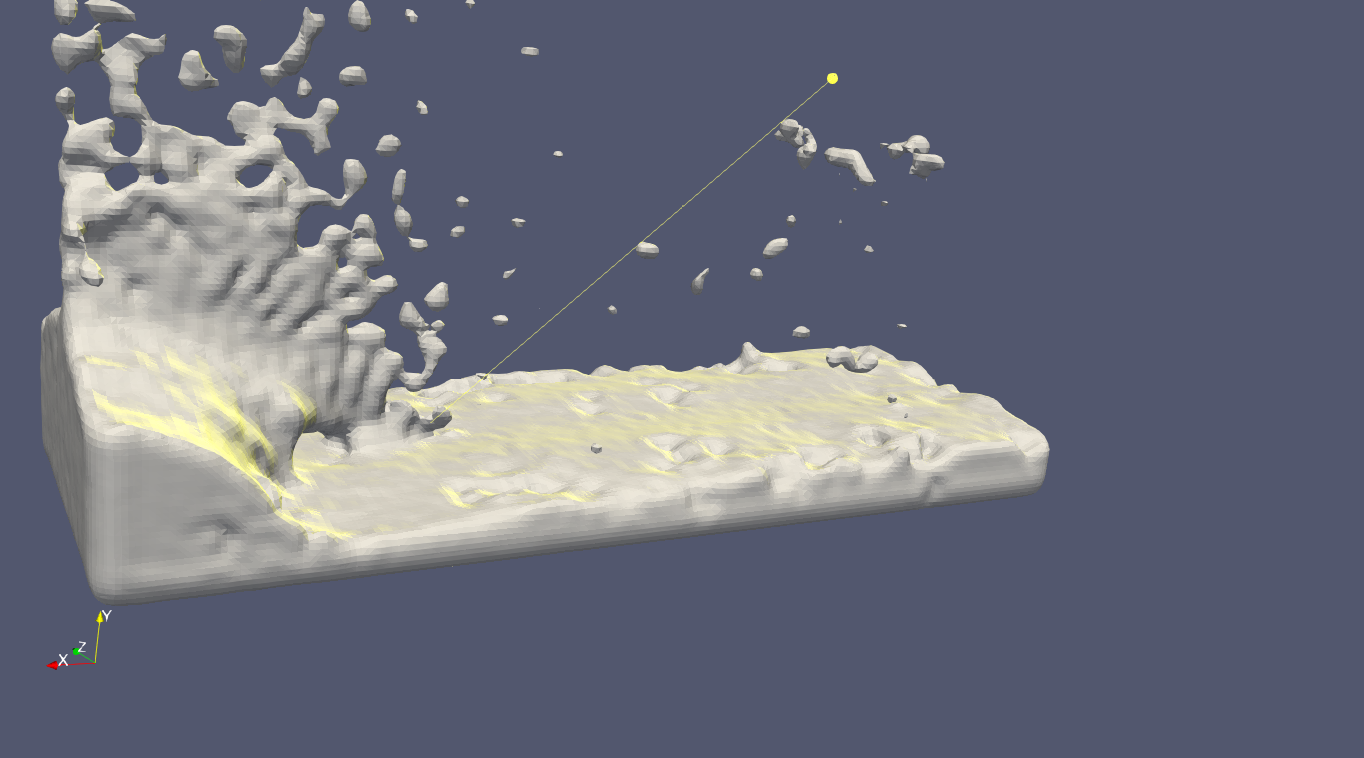
\includegraphics[width=\textwidth]{figures/DenvityBlurredSplashArea2.png}
			\caption{Density based surface reconstruction}
		\end{subfigure}
	\end{center}
	\caption{Comparison of original reconstruction method and blurred reconstruction with application of smoothing factor}
	\label{fig:blur_thin_area_with_sf}
\end{figure}

